\chapter{Frontend}

\section{Arquitectura del Frontend}

El frontend es una \textit{Single Page Application} (SPA) construida con tecnolog\'ia web est\'andar: HTML5, CSS3 y JavaScript vanilla. No utiliza frameworks de JavaScript como React, Angular o Vue, lo que facilita el despliegue y reduce dependencias. La aplicaci\'on utiliza un enrutador casero basado en el hash de la URL (\texttt{window.location.hash}) para la navegaci\'on entre secciones.

\subsection{Estructura de Archivos}

\begin{verbatim}
src/main/resources/static/
  |-- index.html         # Pagina principal SPA (+600 lineas)
  |-- css/
  |   |-- app.css        # Estilos con 8 temas mediante variables CSS (+670 lineas)
  |-- js/
      |-- api.js         # Cliente HTTP con autenticacion JWT (+220 lineas)
      |-- app.js         # Logica principal: routing, modulos, CRUDs (+1590 lineas)
      |-- vet-extras.js  # Sistema de temas y utilidades (+110 lineas)
\end{verbatim}

\section{Pantalla de Login}

La pantalla de inicio de sesi\'on presenta un dise\~no de dos columnas con iconos de mascotas animados (CSS animations), un formulario de login con selecci\'on de tipo (Personal/Cliente) y una pesta\~na para agendar citas p\'ublicamente sin autenticaci\'on.

\begin{figure}[H]
    \centering
    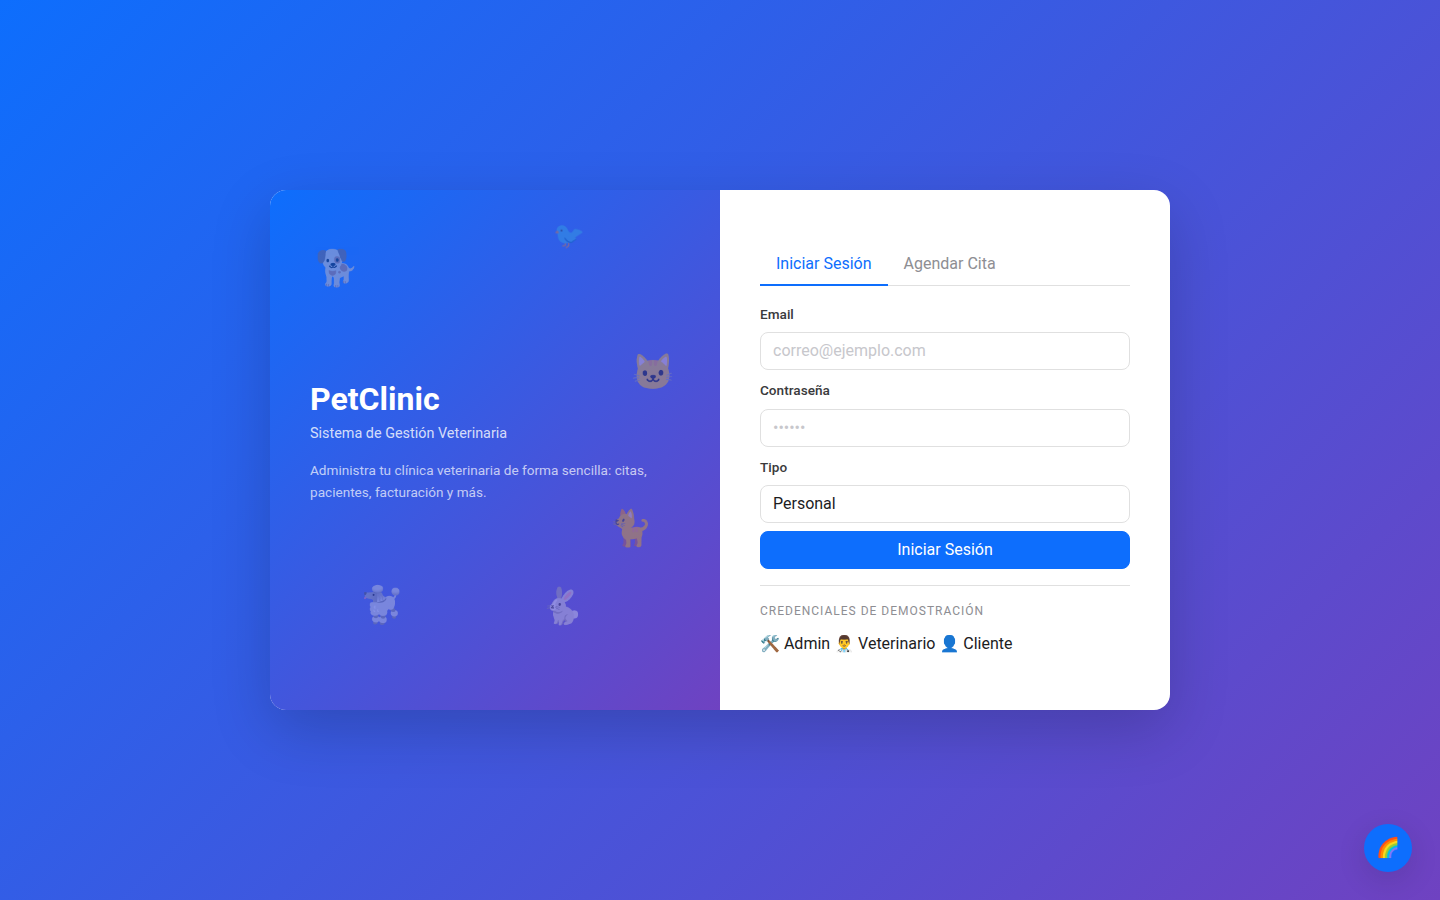
\includegraphics[width=0.8\textwidth]{images/01-login}
    \caption{Pantalla de inicio de sesi\'on con formulario y opci\'on de agenda p\'ublica}
    \label{fig:login}
\end{figure}

\section{Dashboard}

El dashboard muestra 7 tarjetas con estad\'isticas clave del sistema en tiempo real: total de clientes, mascotas, veterinarios, citas hoy, citas pendientes, pacientes hospitalizados y medicamentos con stock bajo. Los datos se cargan mediante \texttt{apiGet('/api/medico/dashboard')} al entrar a la secci\'on.

\begin{figure}[H]
    \centering
    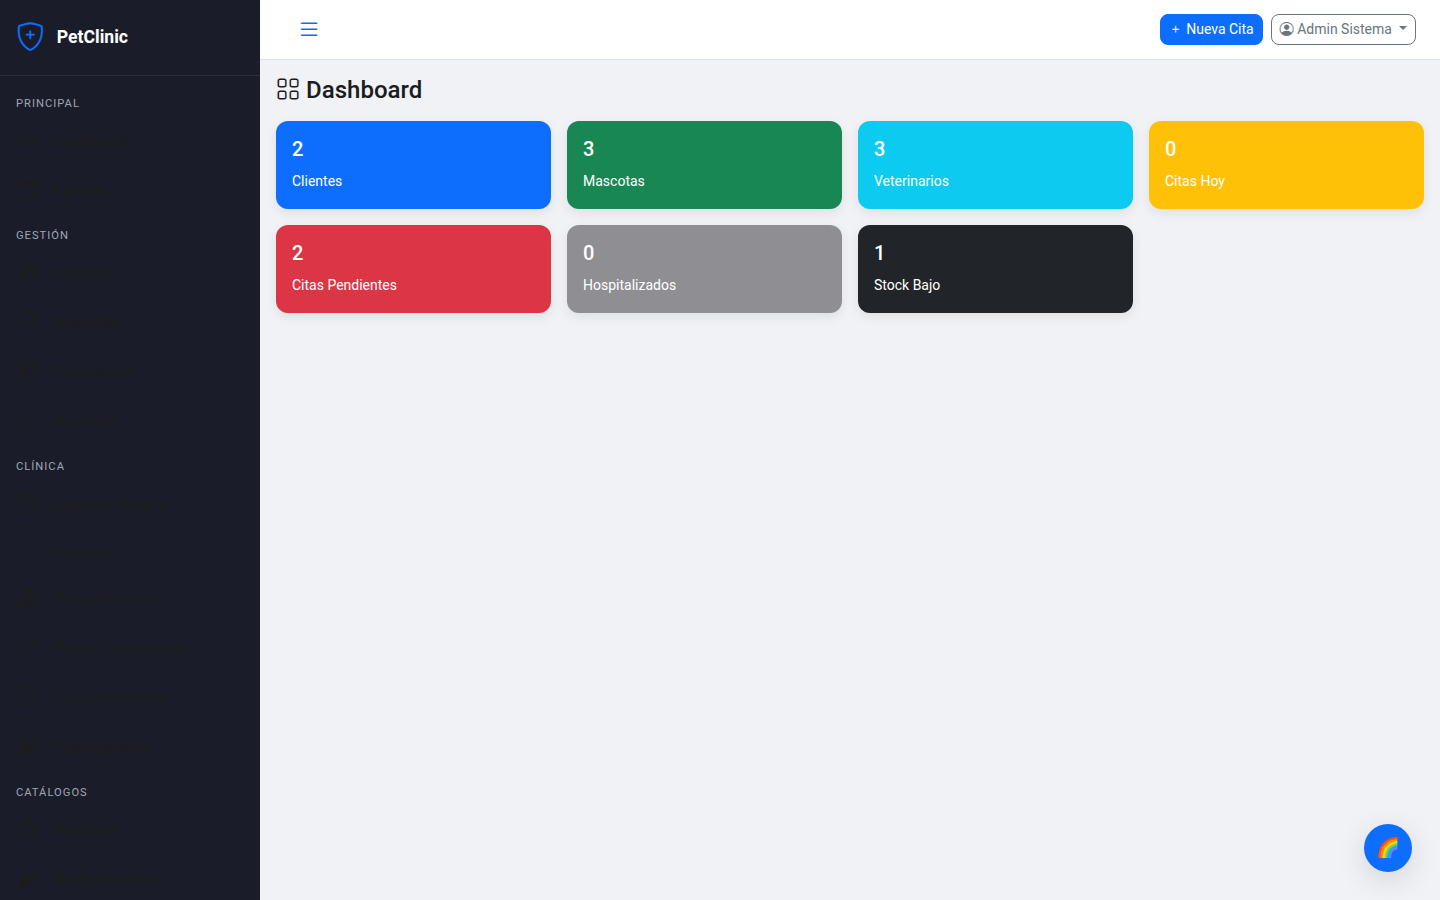
\includegraphics[width=0.9\textwidth]{images/02-dashboard}
    \caption{Dashboard principal con 7 tarjetas de estad\'isticas}
    \label{fig:dashboard2}
\end{figure}

\section{Agenda de Citas}

Utiliza FullCalendar 6 con vistas mensual, semanal y diaria. Soporta arrastrar y soltar para reprogramar citas, codificaci\'on por colores seg\'un el estado (verde=Completada, azul=Programada, amarillo=Confirmada, rojo=Cancelada), y actualizaciones en tiempo real mediante WebSocket.

\begin{lstlisting}[language=JavaScript, caption=Inicializaci\'on de FullCalendar]
const calendar = new FullCalendar.Calendar(calendarEl, {
    plugins: [dayGridPlugin, timeGridPlugin, interactionPlugin],
    headerToolbar: {
        left: 'prev,next today',
        center: 'title',
        right: 'dayGridMonth,timeGridWeek,timeGridDay'
    },
    editable: true,
    events: function(info, successCallback) {
        apiGet('/api/medico/citas').then(data => {
            successCallback(data.map(cita => ({
                id: cita.id,
                title: cita.mascotaNombre + ' - ' + cita.motivo,
                start: cita.fechaHoraInicio,
                end: cita.fechaHoraFin,
                backgroundColor: coloresEstado[cita.estado],
                extendedProps: { estado: cita.estado }
            })));
        });
    },
    eventDrop: function(info) {
        apiPut('/api/medico/citas/' + info.event.id + '/reprogramar', {
            fechaHoraInicio: info.event.start.toISOString(),
            fechaHoraFin: info.event.end.toISOString()
        });
    }
});
calendar.render();
\end{lstlisting}

\begin{figure}[H]
    \centering
    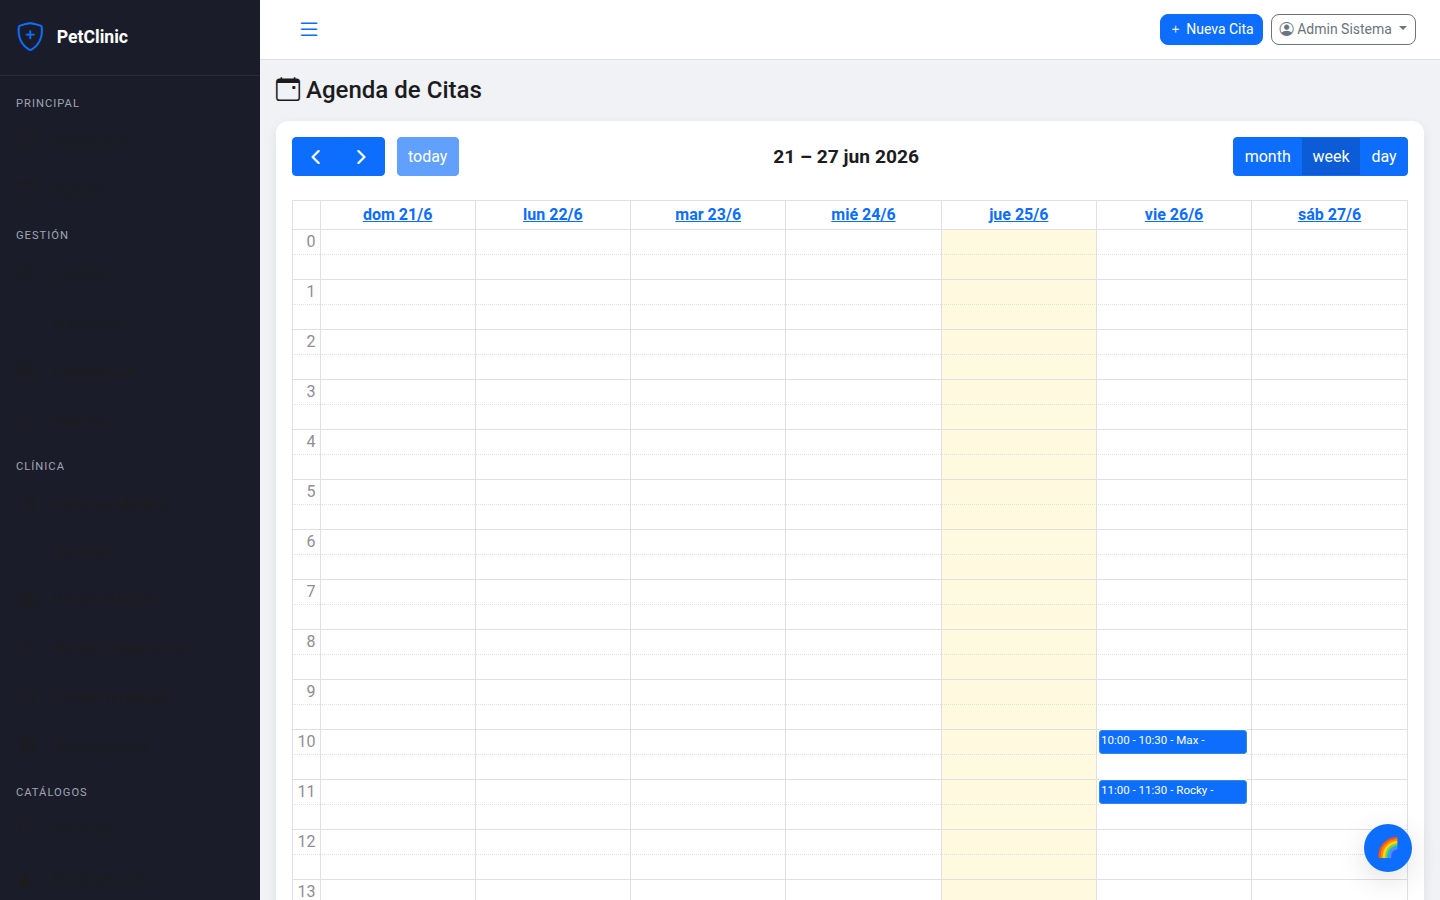
\includegraphics[width=0.9\textwidth]{images/03-agenda}
    \caption{Agenda de citas con FullCalendar en vista mensual}
    \label{fig:agenda}
\end{figure}

\begin{figure}[H]
    \centering
    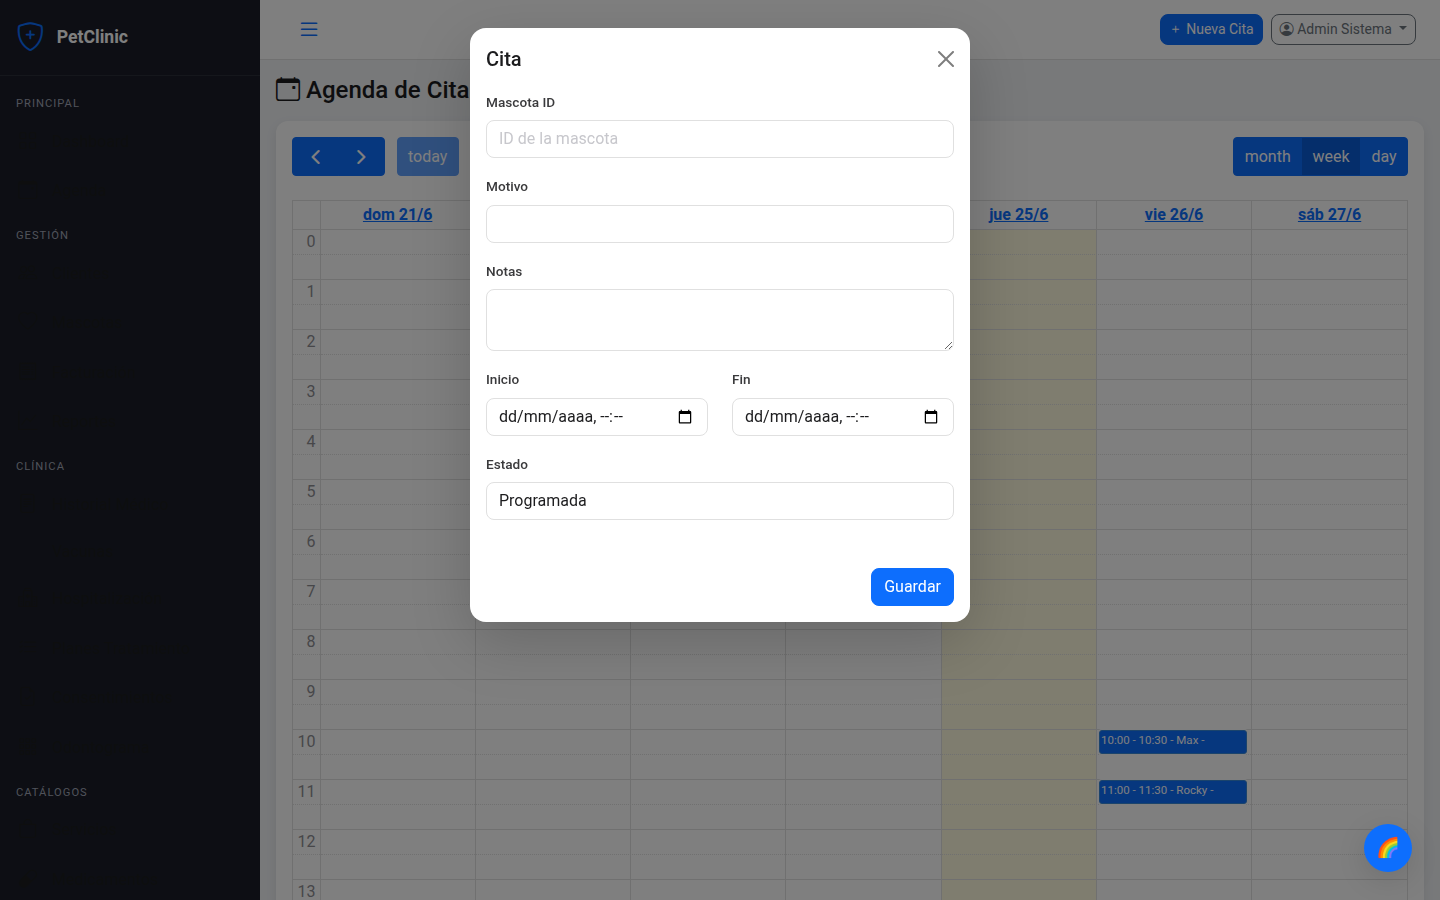
\includegraphics[width=0.6\textwidth]{images/20-modal-cita}
    \caption{Modal de creaci\'on/edici\'on de cita}
    \label{fig:modal-cita}
\end{figure}

\section{Gesti\'on de Clientes y Mascotas}

El m\'odulo de clientes presenta una tabla con b\'usqueda de texto libre, CRUD completo y vista detallada con mascotas asociadas. El m\'odulo de mascotas incluye informaci\'on detallada como especie, raza, peso, alergias y condiciones m\'edicas. Ambos m\'odulos utilizan modales Bootstrap para los formularios de creaci\'on/edici\'on.

\begin{figure}[H]
    \centering
    \begin{subfigure}[b]{0.48\textwidth}
        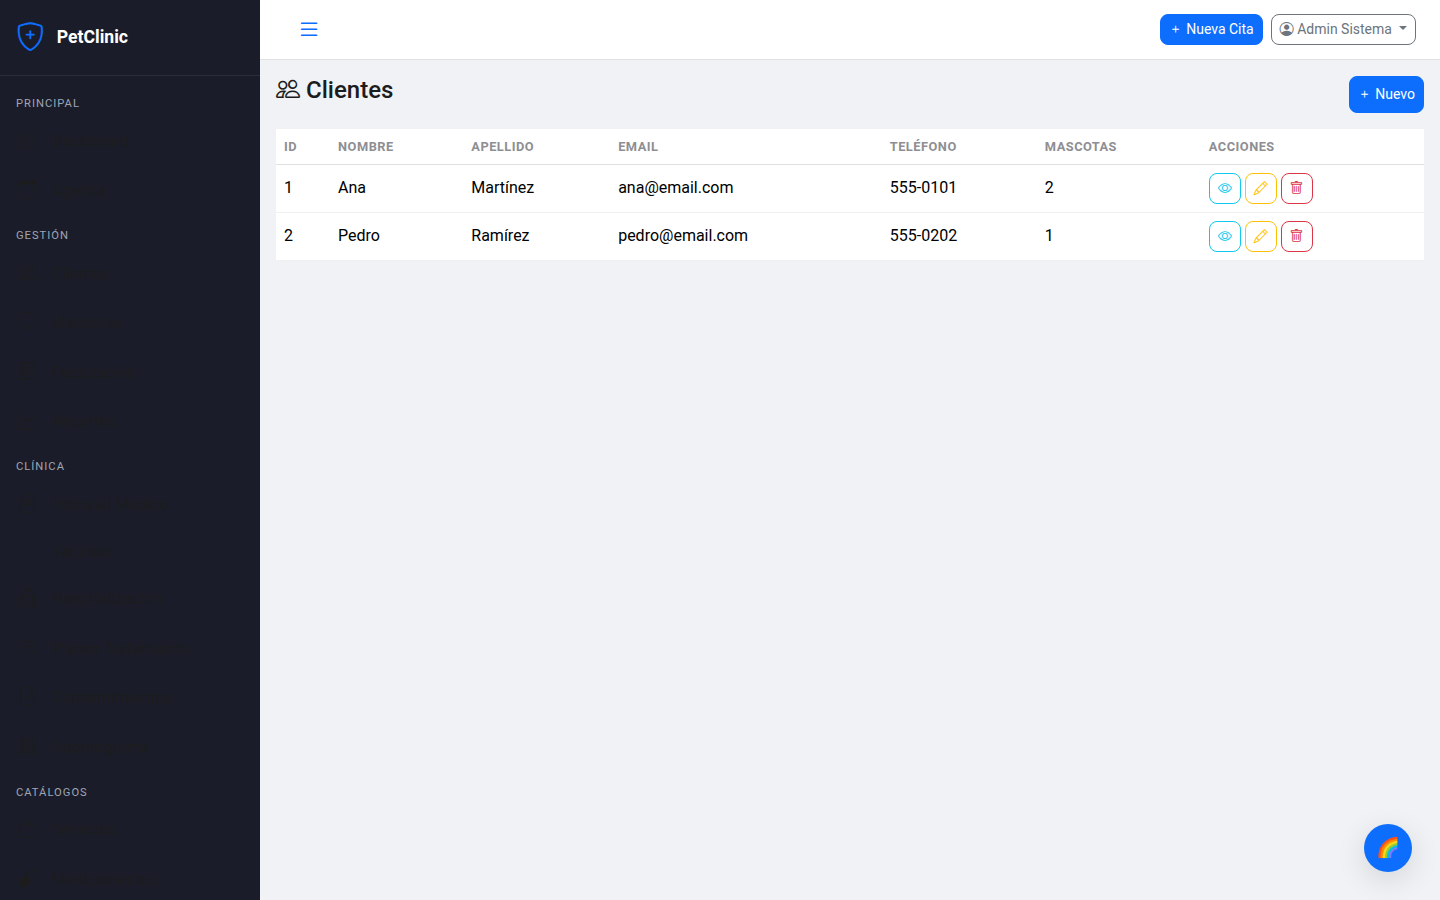
\includegraphics[width=\textwidth]{images/04-clientes}
        \caption{Listado de clientes con b\'usqueda}
    \end{subfigure}
    \hfill
    \begin{subfigure}[b]{0.48\textwidth}
        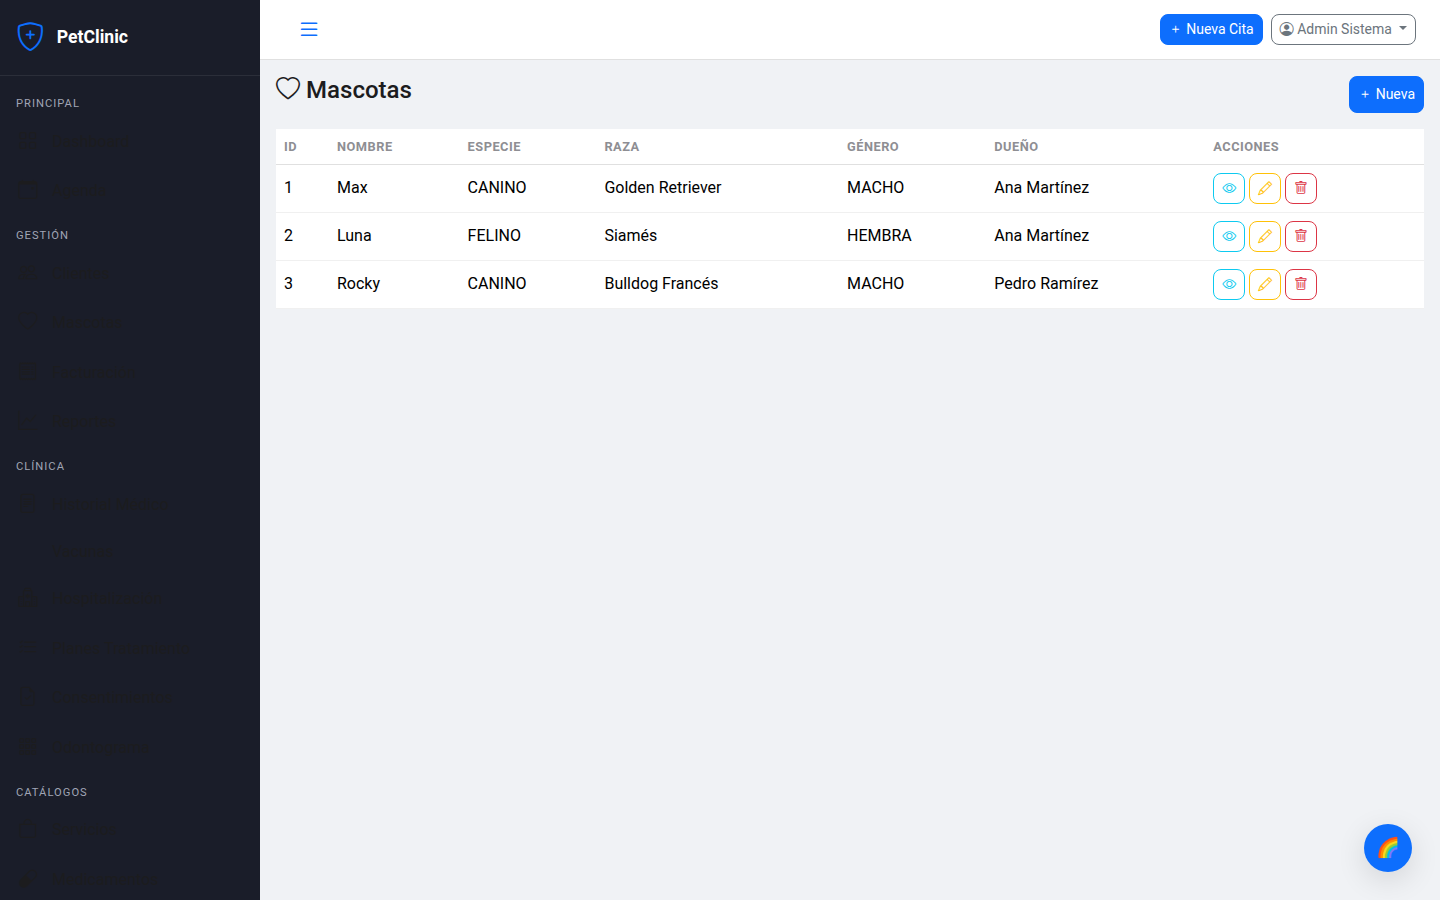
\includegraphics[width=\textwidth]{images/05-mascotas}
        \caption{Listado de mascotas por cliente}
    \end{subfigure}
    \caption{M\'odulos de clientes y mascotas}
    \label{fig:crm}
\end{figure}

\section{Facturaci\'on}

El m\'odulo de facturaci\'on permite crear facturas con items din\'amicos (servicios y medicamentos), c\'alculo autom\'atico de subtotales y totales, descuento autom\'atico de stock, registro de pagos parciales y generaci\'on de PDF con iText 7.

\begin{lstlisting}[language=JavaScript, caption=Creaci\'on de factura con items din\'amicos]
async function guardarFactura() {
    const detalles = [];
    document.querySelectorAll('#detalles-factura .item-row').forEach(row => {
        const tipoItem = row.querySelector('.tipo-item').value;
        const servicioId = row.querySelector('.servicio-id')?.value;
        const medicamentoId = row.querySelector('.medicamento-id')?.value;
        const cantidad = parseInt(row.querySelector('.cantidad').value);
        const precio = parseFloat(row.querySelector('.precio-unitario').value);

        detalles.push({
            tipoItem, servicioId, medicamentoId,
            descripcionLinea: row.querySelector('.descripcion').value,
            cantidad, precioUnitario: precio
        });
    });

    const data = await apiPost('/api/medico/facturas', {
        clienteId: parseInt(document.getElementById('cliente-factura').value),
        detalles: detalles
    });

    toast('Factura creada exitosamente', 'success');
    cargarFacturas();
}
\end{lstlisting}

\begin{figure}[H]
    \centering
    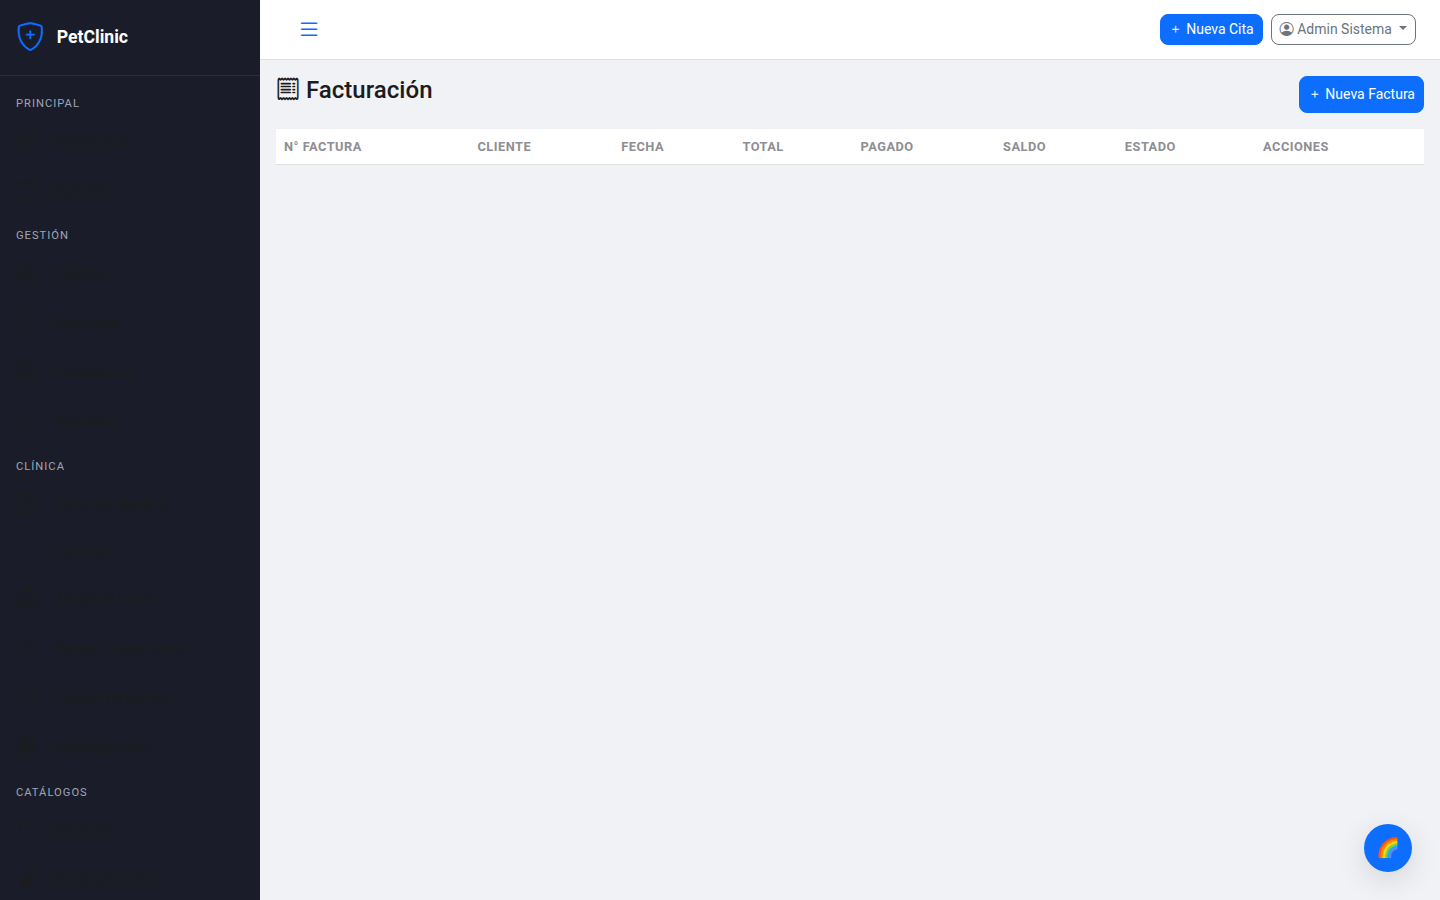
\includegraphics[width=0.9\textwidth]{images/06-facturacion}
    \caption{M\'odulo de facturaci\'on con items din\'amicos}
    \label{fig:facturacion}
\end{figure}

\section{Reportes}

Utiliza Chart.js para mostrar gr\'aficos de ingresos por per\'iodo con opci\'on de descarga en Excel generado con Apache POI en el backend.

\begin{lstlisting}[language=JavaScript, caption=Renderizado de gr\'afico de ingresos con Chart.js]
async function cargarReporte() {
    const data = await apiGet('/api/medico/reportes/ingresos' +
        '?inicio=' + document.getElementById('fecha-inicio').value +
        '&fin=' + document.getElementById('fecha-fin').value);

    new Chart(document.getElementById('chart-ingresos'), {
        type: 'bar',
        data: {
            labels: data.map(d => d.fecha),
            datasets: [{
                label: 'Ingresos ($)',
                data: data.map(d => d.total),
                backgroundColor: 'rgba(54, 162, 235, 0.5)',
                borderColor: 'rgba(54, 162, 235, 1)',
                borderWidth: 1
            }]
        },
        options: {
            responsive: true,
            plugins: {
                legend: { display: true },
                tooltip: { callbacks: {
                    label: ctx => '$' + ctx.parsed.y.toFixed(2)
                }}
            }
        }
    });
}
\end{lstlisting}

\begin{figure}[H]
    \centering
    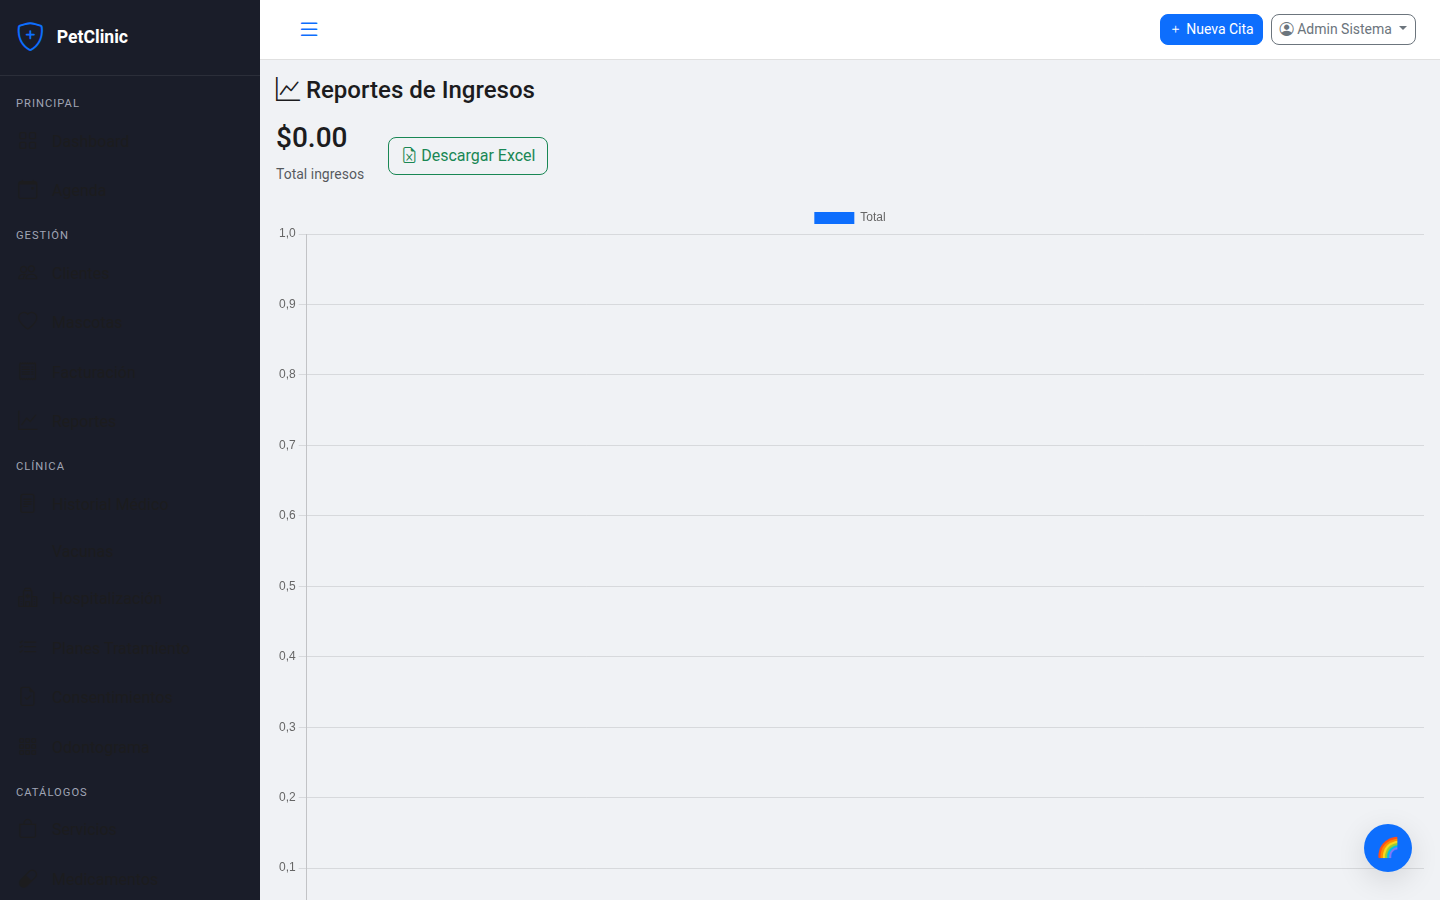
\includegraphics[width=0.9\textwidth]{images/07-reportes}
    \caption{Reportes de ingresos con Chart.js}
    \label{fig:reportes}
\end{figure}

\section{Odontograma Canino}

El odontograma es un diagrama dental interactivo para caninos con 42 dientes numerados seg\'un la f\'ormula dental canina (I 3/3, C 1/1, P 4/4, M 2/3). Permite seleccionar el estado de cada diente (Sano, T\'artaro, Caries, Fractura, Ausente, Periodontal, Obturado, Endodoncia) haciendo clic en el diente correspondiente. El estado se persiste en la base de datos y se pueden tener m\'ultiples odontogramas por mascota (uno por consulta).

\begin{figure}[H]
    \centering
    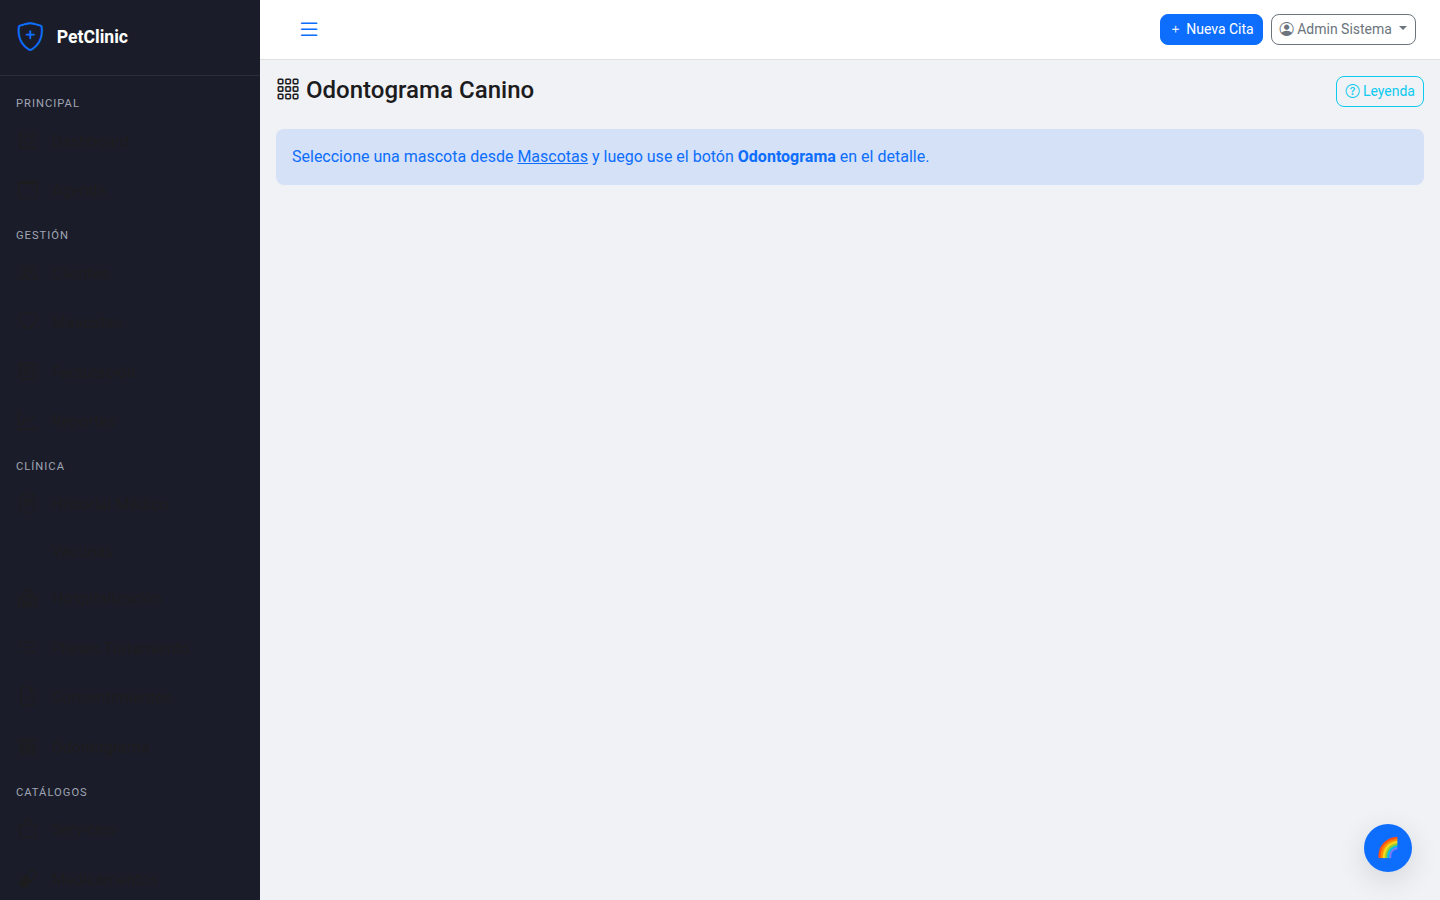
\includegraphics[width=0.9\textwidth]{images/13-odontograma}
    \caption{Odontograma canino interactivo con 42 dientes y 8 estados}
    \label{fig:odontograma}
\end{figure}

\section{Portal del Cliente}

El portal del cliente permite a los due\~nos de mascotas consultar sus citas, facturas e historial m\'edico de manera autogestionada, sin necesidad de contacto con el personal de la cl\'inica.

\begin{figure}[H]
    \centering
    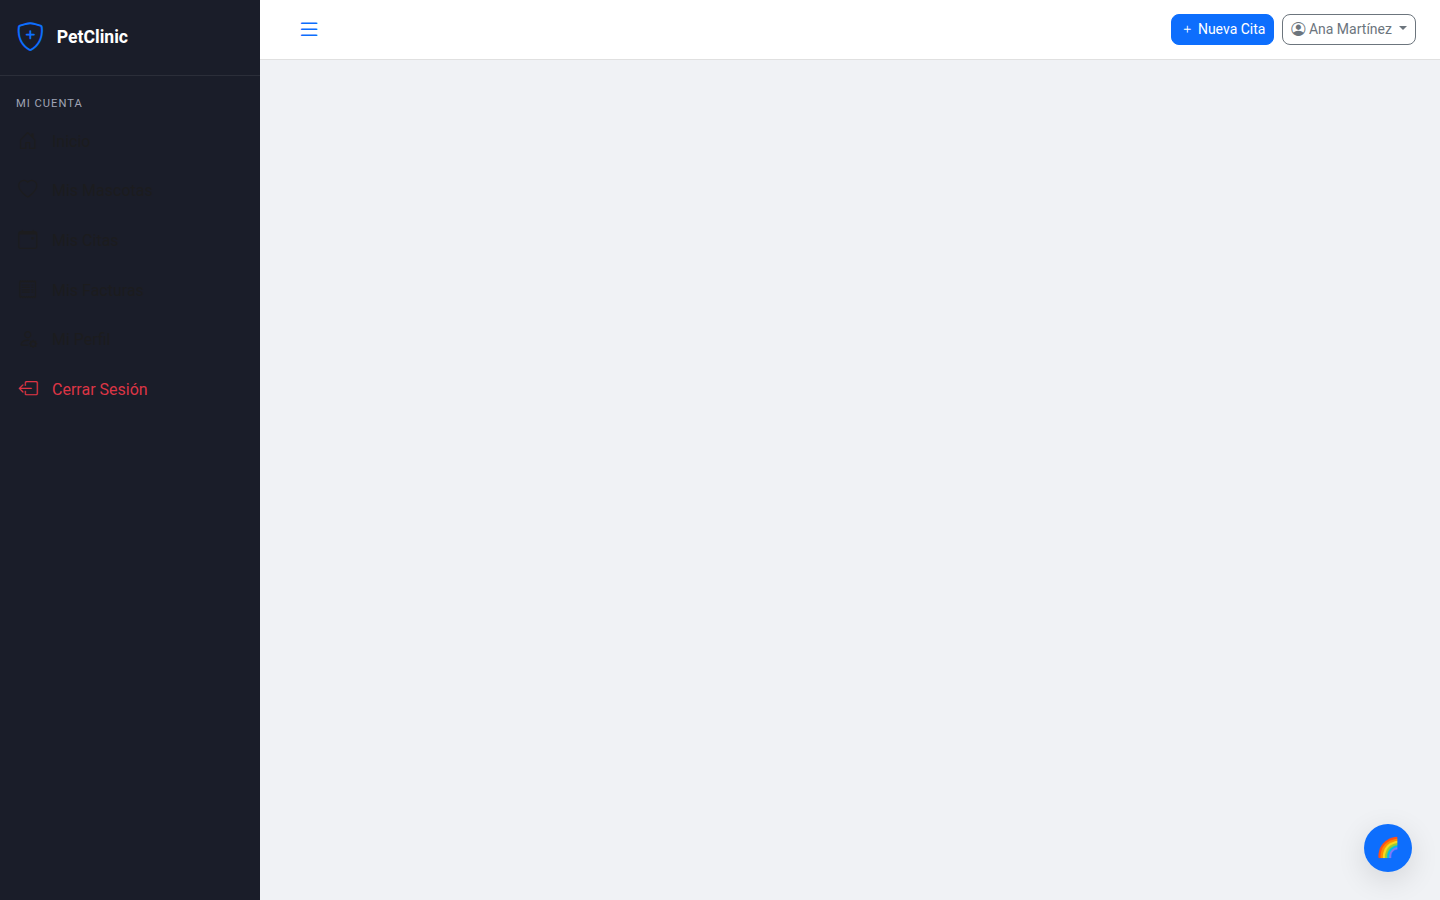
\includegraphics[width=0.9\textwidth]{images/19-portal-cliente}
    \caption{Portal del cliente con citas, mascotas y facturas}
    \label{fig:portal}
\end{figure}

\section{Sistema de Temas}

El sistema incluye 8 temas de color que se pueden cambiar en tiempo real sin recargar la p\'agina mediante el bot\'on flotante en la esquina inferior derecha:

\begin{itemize}
    \item \textbf{Light:} Tema claro predeterminado con fondo blanco y texto oscuro.
    \item \textbf{Dark:} Modo oscuro con fondo \#1a1a2e y texto claro.
    \item \textbf{Terracota:} Tonos tierra c\'alidos con acentos en terracota.
    \item \textbf{Blue Pro:} Azul profesional corporativo.
    \item \textbf{Pink:} Acento rosa para interfaces m\'as suaves.
    \item \textbf{Purple:} Acento p\'urpura con tonos violeta.
    \item \textbf{Olive:} Tonos verdes oliva.
    \item \textbf{Burn (Sunset):} \'Ambar oscuro con degradados de atardecer.
\end{itemize}

Los temas se implementan mediante variables CSS (\textit{Custom Properties}) y se persisten en \texttt{localStorage}. Al cambiar de tema, se actualiza la variable \texttt{data-theme} en el elemento \texttt{<html>} y FullCalendar se refresca autom\'aticamente.

\section{API Cliente (api.js)}

El m\'odulo \texttt{api.js} encapsula toda la comunicaci\'on con el backend HTTP mediante fetch API con manejo centralizado de errores:

\begin{lstlisting}[language=JavaScript, caption=Cliente HTTP con autenticaci\'on JWT]
const API_BASE = '/api';

function getToken() { return localStorage.getItem('vet_token'); }
function getUser() { return JSON.parse(localStorage.getItem('vet_user')||'{}'); }

function authHeaders() {
    return {
        'Content-Type': 'application/json',
        'Authorization': 'Bearer ' + getToken()
    };
}

async function apiGet(path) {
    const res = await fetch(API_BASE + path, { headers: authHeaders() });
    if (!res.ok) {
        const err = await res.json().catch(() => ({}));
        throw new Error(err.error || 'Error ' + res.status);
    }
    return res.json();
}

async function apiPost(path, body) {
    const res = await fetch(API_BASE + path, {
        method: 'POST', headers: authHeaders(),
        body: JSON.stringify(body)
    });
    if (!res.ok) throw new Error((await res.json()).error);
    return res.json();
}

async function apiPut(path, body) {
    const res = await fetch(API_BASE + path, {
        method: 'PUT', headers: authHeaders(),
        body: JSON.stringify(body)
    });
    if (!res.ok) throw new Error((await res.json()).error);
    return res.json();
}

async function apiDelete(path) {
    const res = await fetch(API_BASE + path, {
        method: 'DELETE', headers: authHeaders()
    });
    if (!res.ok) throw new Error((await res.json()).error);
    return res.json();
}

function fmt(num) { return '$' + Number(num||0).toFixed(2); }

function toast(msg, type) {
    const el = document.createElement('div');
    el.className = 'toast show position-fixed bottom-0 end-0 m-3';
    el.innerHTML = '<div class="toast-header bg-' + type + ' text-white">'
        + '<strong>' + type.toUpperCase() + '</strong>'
        + '<button type="button" class="btn-close btn-close-white" '
        + 'data-bs-dismiss="toast"></button></div>'
        + '<div class="toast-body">' + msg + '</div>';
    document.body.appendChild(el);
    setTimeout(() => el.remove(), 3000);
}
\end{lstlisting}
